\chapter{Implementation}
\label{ch:implementation}
\newpage

In this chapter, details of the implementation practical part of the study is discussed. The architecture, modules, development tools, installation, and configurations of such part are the main role of this chapter.    
\section {Architecture}
%The work here uses SANSA~\cite{lehmann-2017-sansa-iswc,iermilov-2017-sansa-iswc-demo}, an open source\url{https://github.com/SANSA-Stack} \emph{data flow processing engine} for performing distributed computation over large-scale RDF datasets. It provides data distribution, communication, and fault tolerance for manipulating massive RDF graphs and applying machine learning algorithms on the data at scale.
	\begin{figure}[ht]
	\begin{center}
		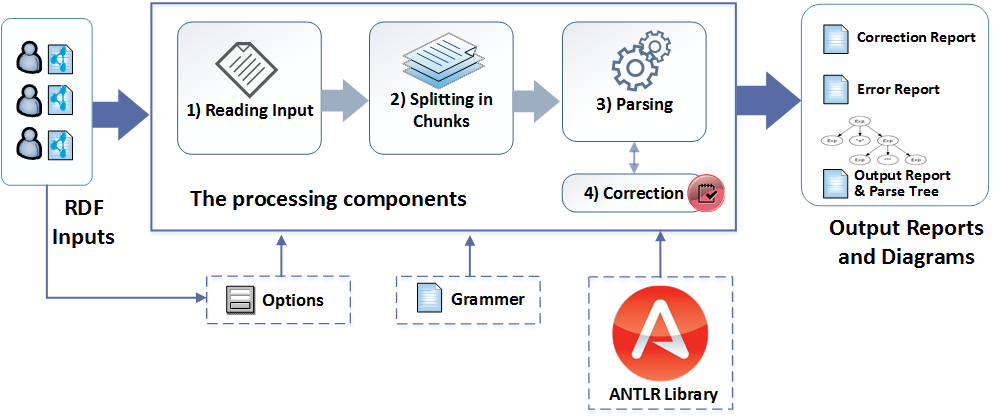
\includegraphics[scale=0.6,angle=0]{images/Architecture}
		\caption{The proposed solution architecture}
		\label{Fig:Architecture}
	\end{center}
\end{figure}
\section {Modules} 
\section{Tools}
\subsection{Hardware}
\subsection{Software}

\section{Installation and Configurations}











